\documentclass[12pt,a4paper]{article}
% Estilo compartido para informes. Compilar con LuaLaTeX desde tp1/.
\usepackage[spanish,es-nodecimaldot]{babel}
\usepackage{fontspec}
\setmainfont{Montserrat-Medium.ttf}[
  Path=../assets/fonts/,
  BoldFont=Montserrat-Bold.ttf,
  ItalicFont=Montserrat-MediumItalic.ttf]
\usepackage[a4paper,margin=2.5cm,headheight=16pt]{geometry}
\usepackage{xcolor,graphicx,booktabs,tabularx}
\usepackage{float}
\usepackage{titlesec,fancyhdr,enumitem,caption}
\usepackage{ragged2e}
\usepackage{hyperref}
\definecolor{verde}{HTML}{1D4036}
\definecolor{bronce}{HTML}{D38129}
\definecolor{rosa}{HTML}{D88E77}
\definecolor{calido}{HTML}{EFE4D8}
\definecolor{grafito}{HTML}{1D1D1D}
\hypersetup{colorlinks=true,linkcolor=verde,urlcolor=verde,
  pdftitle={TP1 - Instalación de máquinas virtuales},pdfsubject={Cyberseguridad}}
\AtBeginDocument{\color{grafito}\RaggedRight\fontsize{12}{14.4}\selectfont}
\setlength{\parindent}{0pt}
\setlength{\parskip}{7pt}
\setlist[itemize]{leftmargin=*,itemsep=7pt,topsep=4pt}
\setlist[enumerate]{leftmargin=*,itemsep=6pt}
\titleformat{\section}{\color{verde}\bfseries\fontsize{18}{21.6}\selectfont}{\thesection}{0.65em}{}
\titleformat{\subsection}{\color{verde}\bfseries\large}{\thesubsection}{0.65em}{}
\titleformat{\subsubsection}{\color{verde}\bfseries}{\thesubsubsection}{0.65em}{}
\titlespacing*{\section}{0pt}{16pt}{8pt}
\titlespacing*{\subsection}{0pt}{12pt}{5pt}
\titlespacing*{\subsubsection}{0pt}{10pt}{4pt}
\setcounter{tocdepth}{2}
\pagestyle{fancy}
\fancyhf{}
\fancyhead[L]{\small\color{verde}FCEFyN | UNC}
\fancyhead[R]{\small\color{verde}\materia\ · TP \numeroTP}
\fancyfoot[L]{\scriptsize Informe de laboratorio}
\fancyfoot[R]{\small\thepage}
\renewcommand{\headrulewidth}{0.4pt}
\captionsetup{font=small,labelfont=bf,justification=raggedright,singlelinecheck=false,hypcap=false}
\newcommand{\pendiente}[1]{\par{\small\color{verde}\textbf{Por completar.} #1\par}}
% Si falta una captura se muestra un espacio reservado; no impide compilar.
\newcommand{\captura}[2]{%
  \par\smallskip\begingroup\centering
  \IfFileExists{figuras/#1}{%
    \includegraphics[width=\linewidth,height=5cm,keepaspectratio]{figuras/#1}%
  }{%
    \setlength{\fboxsep}{10pt}%
    \fcolorbox{bronce}{calido}{\parbox[c][1.25cm][c]{\dimexpr\linewidth-2\fboxsep-2\fboxrule\relax}{%
      \centering\small Captura pendiente\par\texttt{\detokenize{#1}}}}%
  }%
  \captionof{figure}{#2}\par\endgroup\smallskip
}

\usepackage{xurl}

\newcommand{\materia}{Cyberseguridad}
\newcommand{\numeroTP}{3}
\newcommand{\tituloTP}{Expresiones regulares}
\newcommand{\estudiante}{Brigido Tomas Andres}
\newcommand{\legajo}{38481096}
\newcommand{\carrera}{ICOMP}
\newcommand{\docente}{Javier A. Jorge}


% Metadatos específicos del TP3 y capturas en img/.
\hypersetup{pdftitle={TP3 - Expresiones regulares}}
\renewcommand{\captura}[2]{%
  \begin{figure}[H]
    \centering
    \IfFileExists{img/#1}{%
      \includegraphics[width=0.85\linewidth,height=5cm,keepaspectratio]{img/#1}%
    }{%
      \setlength{\fboxsep}{10pt}%
      \fcolorbox{bronce}{calido}{\parbox[c][1.1cm][c]{0.85\linewidth}{%
        \centering\small Captura pendiente\par\texttt{\detokenize{#1}}}}%
    }%
    \caption{#2}
  \end{figure}
}

\begin{document}
\hypersetup{pageanchor=false}
\begin{titlepage}
  
\includegraphics[width=8cm]{../assets/logo-fcefyn-2026.png}
  \vspace{1cm}

  {\color{verde}\small UNIVERSIDAD NACIONAL DE CÓRDOBA\par}
  \vspace{2.1cm}
  {\color{bronce}\bfseries\large TRABAJO PRÁCTICO \numeroTP\par}
  \vspace{0.45cm}
  {\color{verde}\bfseries\fontsize{32}{38.4}\selectfont Expresiones\\regulares\par}
  \vspace{0.65cm}
  {\large \materia\par}
  \vspace{0.8cm}
  {\color{bronce}\rule{2.7cm}{2pt}\par}
  \vfill
  \renewcommand{\arraystretch}{1.45}
  \begin{tabular}{@{}p{3.2cm}p{10cm}@{}}
    Estudiante & \estudiante \\
    Legajo & \legajo \\
    Carrera & \carrera \\
    Docente & \docente \\
  \end{tabular}
  \vfill
  {\small Córdoba, Argentina\par}
\end{titlepage}
\hypersetup{pageanchor=true}

\tableofcontents
\vspace{1cm}
\newpage

\section{Introducción y objetivos}
Este trabajo se centra en el uso de expresiones regulares para buscar
cadenas de texto. La consigna propone completar el tutorial de RegexOne,
describir metacaracteres y patrones, y contrastar las respuestas con un
archivo de registro en CyberOps Workstation.

\begin{itemize}
    \item Reconocer los metacaracteres y su función en una expresión regular.
    \item Interpretar qué cadenas coinciden con los patrones propuestos.
    \item Verificar las interpretaciones mediante búsquedas con \texttt{less}.
\end{itemize}

\section{Paso 1: tutorial y metacaracteres}

\begingroup
\small
\renewcommand{\arraystretch}{1.35}
\begin{tabular}{@{}p{3cm}>{\RaggedRight\arraybackslash}p{12cm}@{}}
\toprule
\textbf{Metacarácter} & \textbf{Descripción} \\
\midrule
\verb|$| & Ancla la coincidencia al final de la línea. \\
\verb|*| & Repite el elemento anterior cero o más veces. \\
\verb|.| & Coincide con un carácter cualquiera, normalmente excepto el salto de línea. \\
\verb|[]| & Define una clase de caracteres: coincide con uno de los incluidos entre los corchetes. \\
\verb|\.| & Coincide con un punto literal. \\
\verb|\d| & Coincide con un dígito. \\
\verb|\D| & Coincide con un carácter que no sea un dígito. \\
\verb|^| & Ancla la coincidencia al inicio de la línea. \\
\verb|{m}| & Repite el elemento anterior exactamente m veces. \\
\verb|{n,m}| & Repite el elemento anterior entre n y m veces, inclusive. \\
\verb!abc|123! & Alternancia: coincide con la cadena \texttt{abc} o con la cadena \texttt{123}. \\
\bottomrule
\end{tabular}
\endgroup

\newpage
\section{Paso 2: interpretación de patrones}
Los ejemplos siguientes ilustran los patrones; las coincidencias del archivo
se registran en el paso 3.

\begingroup
\small
\renewcommand{\arraystretch}{1.65}
\begin{tabular}{@{}p{3.3cm}>{\RaggedRight\arraybackslash}p{7cm}>{\RaggedRight\arraybackslash}p{4.3cm}@{}}
\toprule
\textbf{Patrón} & \textbf{Descripción} & \textbf{Ejemplo} \\
\midrule
\verb|^83| & Coincide con \texttt{83} al inicio de una línea. & \texttt{83} al inicio de \texttt{83.149.9.216} \\
\verb|[A-Z]{2,4}| & Coincide con una secuencia de dos a cuatro letras mayúsculas de A a Z. & \texttt{GET}, \texttt{HTTP} \\
\verb|2015| & Coincide con la secuencia literal \texttt{2015}. & \texttt{2015} \\
\verb|05:22:2[0-9]| & Coincide con \texttt{05:22:2} seguido de un dígito: desde \texttt{05:22:20} hasta \texttt{05:22:29}. & \texttt{05:22:25} \\
\verb|\.com| & Coincide con un punto literal seguido de \texttt{com}. & \texttt{.com} \\
\verb!complete|GET! & Coincide con \texttt{complete} o con \texttt{GET}. & \texttt{complete}, \texttt{GET} \\
\verb|0{4}| & Coincide con cuatro ceros consecutivos. & \texttt{0000} \\
\bottomrule
\end{tabular}
\endgroup

\newpage
\section{Paso 3: verificación en la VM}
\subsection{Apertura del archivo de registro y busqueda de las expresiones}
Dentro de CyberOps Workstation ejecutamos en la terminal:

\begin{verbatim}
cd ~/lab.support.files/
less logstash-tutorial.log
\end{verbatim}

Dentro de \texttt{less}, escribir cada búsqueda y presionar Intro:

\begin{verbatim}
/^83
/[A-Z]{2,4}
/\.com
/0{4}
\end{verbatim}

\begin{figure}[H]
    \centering
    \begin{minipage}[t]{0.48\textwidth}
        \centering
        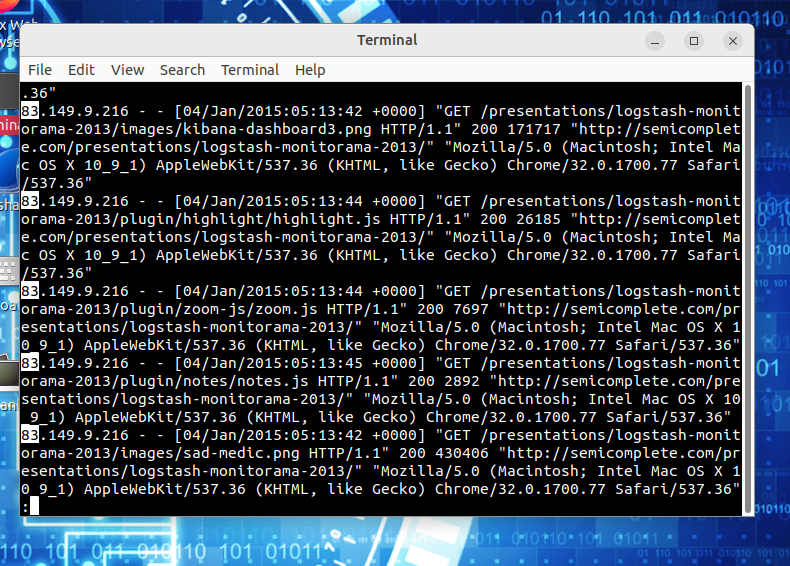
\includegraphics[width=\linewidth]{img/primeraregex.png}
        \caption{Coincidencia del patrón \texttt{\detokenize{^83}}.}
        \label{fig:imagen1}
    \end{minipage}
    \hfill
    \begin{minipage}[t]{0.48\textwidth}
        \centering
        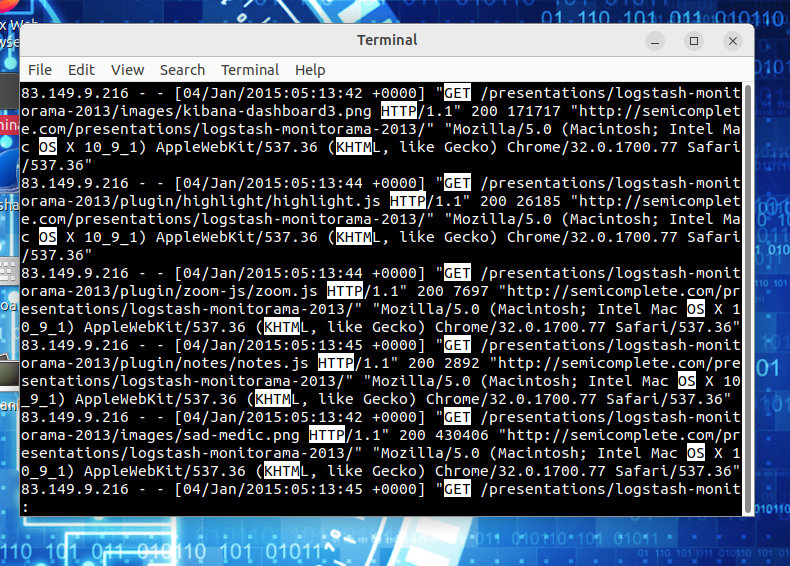
\includegraphics[width=\linewidth]{img/segundaregex.png}
        \caption{Coincidencia del patrón \texttt{\detokenize{[A-Z]{2,4}}}.}
        \label{fig:imagen2}
    \end{minipage}

    \vspace{0.5cm}

    \begin{minipage}[t]{0.48\textwidth}
        \centering
        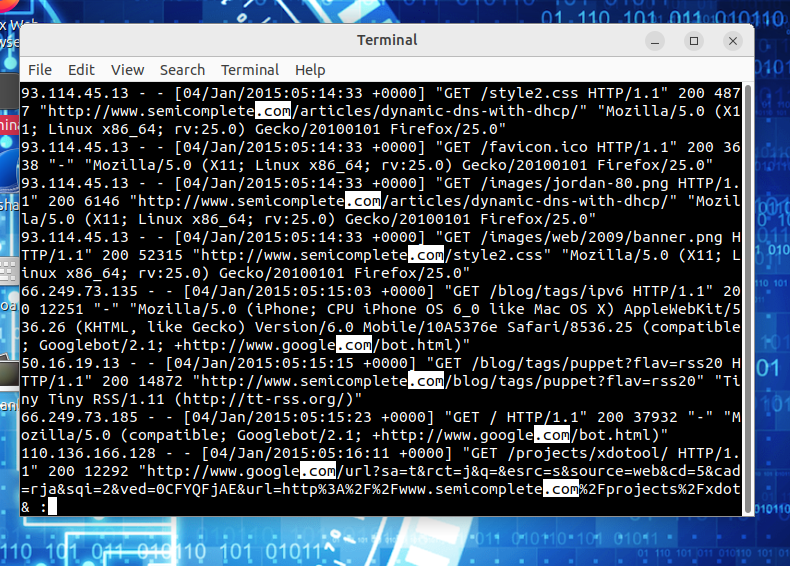
\includegraphics[width=\linewidth]{img/puntocomregex.png}
        \caption{Coincidencia del patrón \texttt{\detokenize{\.com}}.}
        \label{fig:imagen3}
    \end{minipage}
    \hfill
    \begin{minipage}[t]{0.48\textwidth}
        \centering
        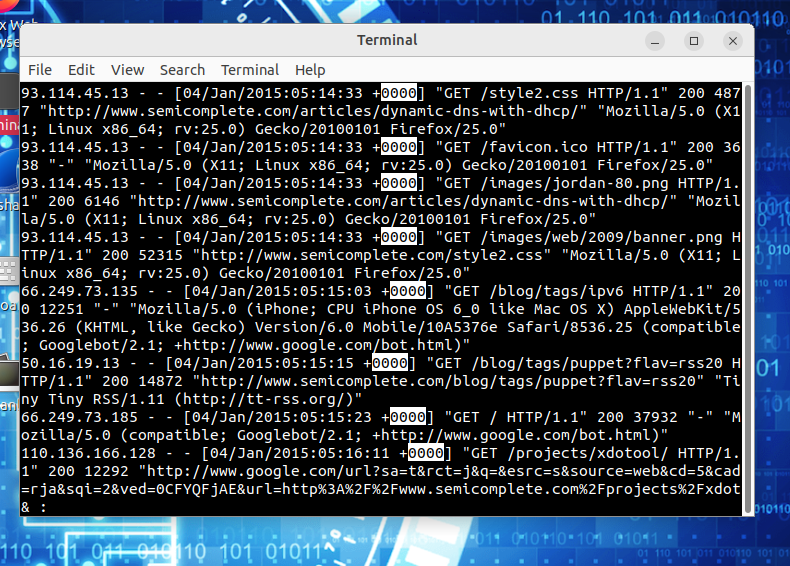
\includegraphics[width=\linewidth]{img/4cerosregex.png}
        \caption{Coincidencia del patrón \texttt{\detokenize{0{4}}}.}
        \label{fig:imagen4}
    \end{minipage}
\end{figure}


\newpage
\section{Referencias}
\begin{enumerate}
    \item Cisco Networking Academy. \textit{Práctica de laboratorio: Tutorial
    de expresiones regulares}. Consigna suministrada en
    \textit{2.A Regular Expression Lab.pdf}, 3 páginas.
    \item RegexOne. \textit{Learn Regular Expressions with simple,
    interactive exercises}. \url{https://regexone.com/}.
    \item FCEFyN, Universidad Nacional de Córdoba. \textit{Manual de
    identidad visual}, 2026. Base del estilo compartido del informe.
\end{enumerate}
\end{document}
